% Figure 5 -- A) Hitchin system for SU(2) QCDs (filled dot: type II irregular,
%             circle: type I irregular, cross: regular; number = integer part of pole order)
%             B) singularity structure of the corresponding AD theory
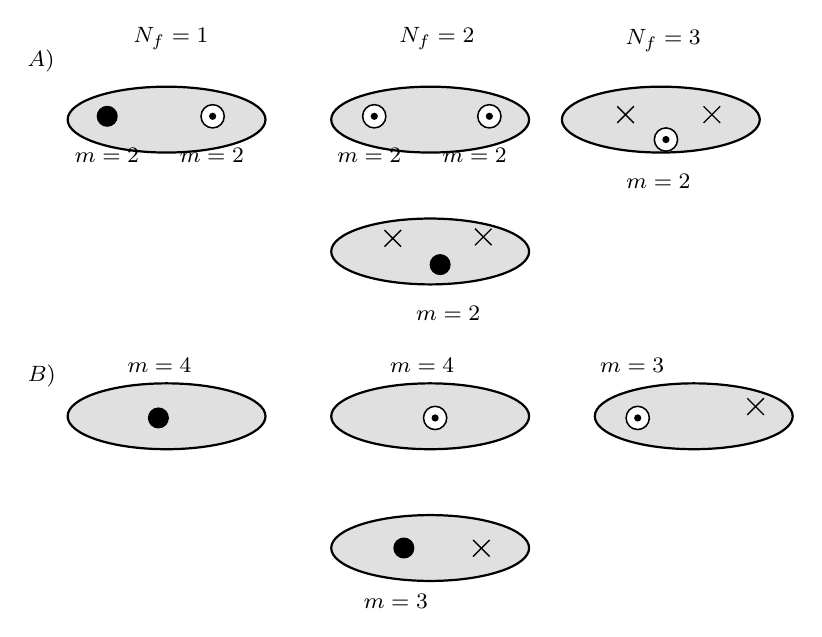
\begin{tikzpicture}[x=1pt,y=1pt,>=stealth,line width=0.5pt,
    ell/.style={draw,fill=black!12,line width=0.8pt}]
  % ================= A) =================
  \node[inner sep=0pt,font=\footnotesize] at (6.9,200.6) {$A)$};
  % N_f = 1
  \draw[ell] (52.25,179.4) ellipse[x radius=35.75pt,y radius=11.9pt];
  \fill (30.8,180.6) circle[radius=3.8pt];
  \draw[line width=0.55pt,fill=white] (68.9,180.6) circle[radius=4.2pt];
  \fill (68.9,180.6) circle[radius=1.3pt];
  \node[inner sep=0pt,font=\footnotesize] at (53.8,208.6) {$N_f=1$};
  \node[inner sep=0pt,font=\footnotesize] at (30.7,166.4) {$m=2$};
  \node[inner sep=0pt,font=\footnotesize] at (68.6,166.4) {$m=2$};
  % N_f = 2
  \draw[ell] (147.5,179.4) ellipse[x radius=35.75pt,y radius=11.9pt];
  \draw[line width=0.55pt,fill=white] (127.3,180.6) circle[radius=4.2pt];
  \fill (127.3,180.6) circle[radius=1.3pt];
  \draw[line width=0.55pt,fill=white] (168.9,180.6) circle[radius=4.2pt];
  \fill (168.9,180.6) circle[radius=1.3pt];
  \node[inner sep=0pt,font=\footnotesize] at (149.9,208.6) {$N_f=2$};
  \node[inner sep=0pt,font=\footnotesize] at (125.5,166.4) {$m=2$};
  \node[inner sep=0pt,font=\footnotesize] at (163.6,166.4) {$m=2$};
  % N_f = 3
  \draw[ell] (230.85,179.4) ellipse[x radius=35.75pt,y radius=11.9pt];
  \draw (215.1,178.2) -- (221.1,184.2);
  \draw (215.1,184.2) -- (221.1,178.2);
  \draw (246.3,178.2) -- (252.3,184.2);
  \draw (246.3,184.2) -- (252.3,178.2);
  \draw[line width=0.55pt,fill=white] (232.7,172.2) circle[radius=4.2pt];
  \fill (232.7,172.2) circle[radius=1.3pt];
  \node[inner sep=0pt,font=\footnotesize] at (231.7,208.0) {$N_f=3$};
  \node[inner sep=0pt,font=\footnotesize] at (230.0,157.0) {$m=2$};
  % second row of A)
  \draw[ell] (147.5,131.75) ellipse[x radius=35.75pt,y radius=11.9pt];
  \draw (131.0,133.5) -- (137.0,139.5);
  \draw (131.0,139.5) -- (137.0,133.5);
  \draw (163.7,134.0) -- (169.7,140.0);
  \draw (163.7,140.0) -- (169.7,134.0);
  \fill (151.1,127.0) circle[radius=3.8pt];
  \node[inner sep=0pt,font=\footnotesize] at (154.0,109.5) {$m=2$};
  % ================= B) =================
  \node[inner sep=0pt,font=\footnotesize] at (7.2,86.7) {$B)$};
  % m = 4 (type II)
  \draw[ell] (52.25,72.2) ellipse[x radius=35.75pt,y radius=11.9pt];
  \fill (49.3,71.6) circle[radius=3.8pt];
  \node[inner sep=0pt,font=\footnotesize] at (49.7,90.5) {$m=4$};
  % m = 4 (type I)
  \draw[ell] (147.5,72.2) ellipse[x radius=35.75pt,y radius=11.9pt];
  \draw[line width=0.55pt,fill=white] (149.3,71.6) circle[radius=4.2pt];
  \fill (149.3,71.6) circle[radius=1.3pt];
  \node[inner sep=0pt,font=\footnotesize] at (144.6,90.5) {$m=4$};
  % m = 3 (type I + regular)
  \draw[ell] (242.75,72.2) ellipse[x radius=35.75pt,y radius=11.9pt];
  \draw[line width=0.55pt,fill=white] (222.5,71.6) circle[radius=4.2pt];
  \fill (222.5,71.6) circle[radius=1.3pt];
  \draw (262.1,72.7) -- (268.1,78.7);
  \draw (262.1,78.7) -- (268.1,72.7);
  \node[inner sep=0pt,font=\footnotesize] at (220.5,90.5) {$m=3$};
  % second row of B)
  \draw[ell] (147.5,24.6) ellipse[x radius=35.75pt,y radius=11.9pt];
  \fill (138,24.6) circle[radius=3.8pt];
  \draw (163.0,21.5) -- (169.0,27.5);
  \draw (163.0,27.5) -- (169.0,21.5);
  \node[inner sep=0pt,font=\footnotesize] at (135.1,5.2) {$m=3$};
\end{tikzpicture}
